%!TEX program = xelatex
%!TEX root = ./thesis.tex
\chapter{Experiments}\label{chap:experiments}

% \yan{How about using the title ``Evaluations''?}
% No, thx.
% \yan{For grammar issues, do you mind using Grammarly \textit{https://app.grammarly.com/} to check your document? Our lab often uses it when writing English papers.}
% Yep, this whole thesis has already been revised on Grammarly.

The GreenEyes model is based on WaveNet and LSTM. Unlike computer vision models, which take 2D images as inputs, the GreenEyes model is trained on 1D sequential data arrays.

To build a data feeding pipeline, we built a slice data generator on the $PM_{2.5}$ IAQI data. Train data pairs as below are fed to the model:

\begin{equation}
\left\{
    \begin{array}{l}
    X_i=[D(t_i),D(t_{i+1}),...,D(t_{i+L-1})] \\
    y_i=P(t_{i+L})
    \end{array}
\right.
\end{equation}

% 实验目的是用window化的 IAQI 数据(注意是iaqi数据,不是原始pm数据)fit手动标注的 IAQI level

Where $D$ denotes the whole $PM_{2.5}$ IAQI data array, $P$ denotes the whole target function, i.e., the polygonized IAQI level we get in the last chapter. It is clear that our model takes a 1D array as input and outputs a scalar.

$L$ denotes the length of the slice when we sample sequences from the $PM_{2.5}$ IAQI data, and $t_i$, $t_{i+1}$ etc. are the discrete-time points. Note that to make the model to be \textbf{causal}, the target value $y_i$ in the train data pair is sampled at time point $t_{i+L}$, which is exactly next to the last time point in $X_i$.

In our experiment, as the total length of the $PM_{2.5}$ IAQI data is 219,989, setting different values for the length of the slice $L$ will firstly lead to variant input size for the GreenEyes model because the input size equals $L$, which will also make the number of training parameters larger or smaller. Secondly, as the length of the whole sequence data is limited, the larger $L$ is, the less the number of total train data is. Number of total train data is $(219,989-L+1)$.

We finally chose 7,200 as the length of the slice for the following reasons:
\begin{enumerate}
    \item 7,200 seconds equals 2 hours in the time axis, and we design the model to predict the next second's IAQI level by previous data within these 2 hours.
    \item The model's size (number of parameters, etc.) w.r.t. the input size of 7,200 is exactly appropriate both for learning and inferring.
\end{enumerate}

\section{Data Sampling and Splitting}

As described above, the number of total train data is $(219,989-L+1)$. When setting $L=7200$, it is 212,790, which is an enormous number when feeding the model. Hence, we introduced the sampling method and set stride when collecting train samples from the original data, and the size will be $\frac{\lfloor 219,989-L+1 \rfloor}{stride}+1$. 

Moreover, we split the data into a training set and validation set, with a validation ratio of 0.2. The number of training/validation samples varies when stride varies. Out experiments use 10, 5, 2 as stride's value and Table \ref{table:N_samples} illustrates the number of training/validation samples.

\begin{table}[!htbp]
    \centering
    \begin{tabular}{|l|l|l|l|l|}
    \hline
    $L$ (The length of the slice) & Stride & $N_{samples}$ & $N_{train}$ & $N_{val}$ \\ \hline
    7200 & 10 & 21280  & 17024  & 4256  \\ \hline
    7200 & 5  & 42559  & 34048  & 8511  \\ \hline
    7200 & 2  & 106396 & 85117  & 21279 \\ \hline
    \end{tabular}
    \caption{The relationship between different strides and number of samples.}
    \label{table:N_samples}
\end{table}

Figure \ref{fig:model_feeding_pipeline} shows the model feeding pipeline of our GreenEyes model during training.

\begin{figure}[!htbp]
    \centering
    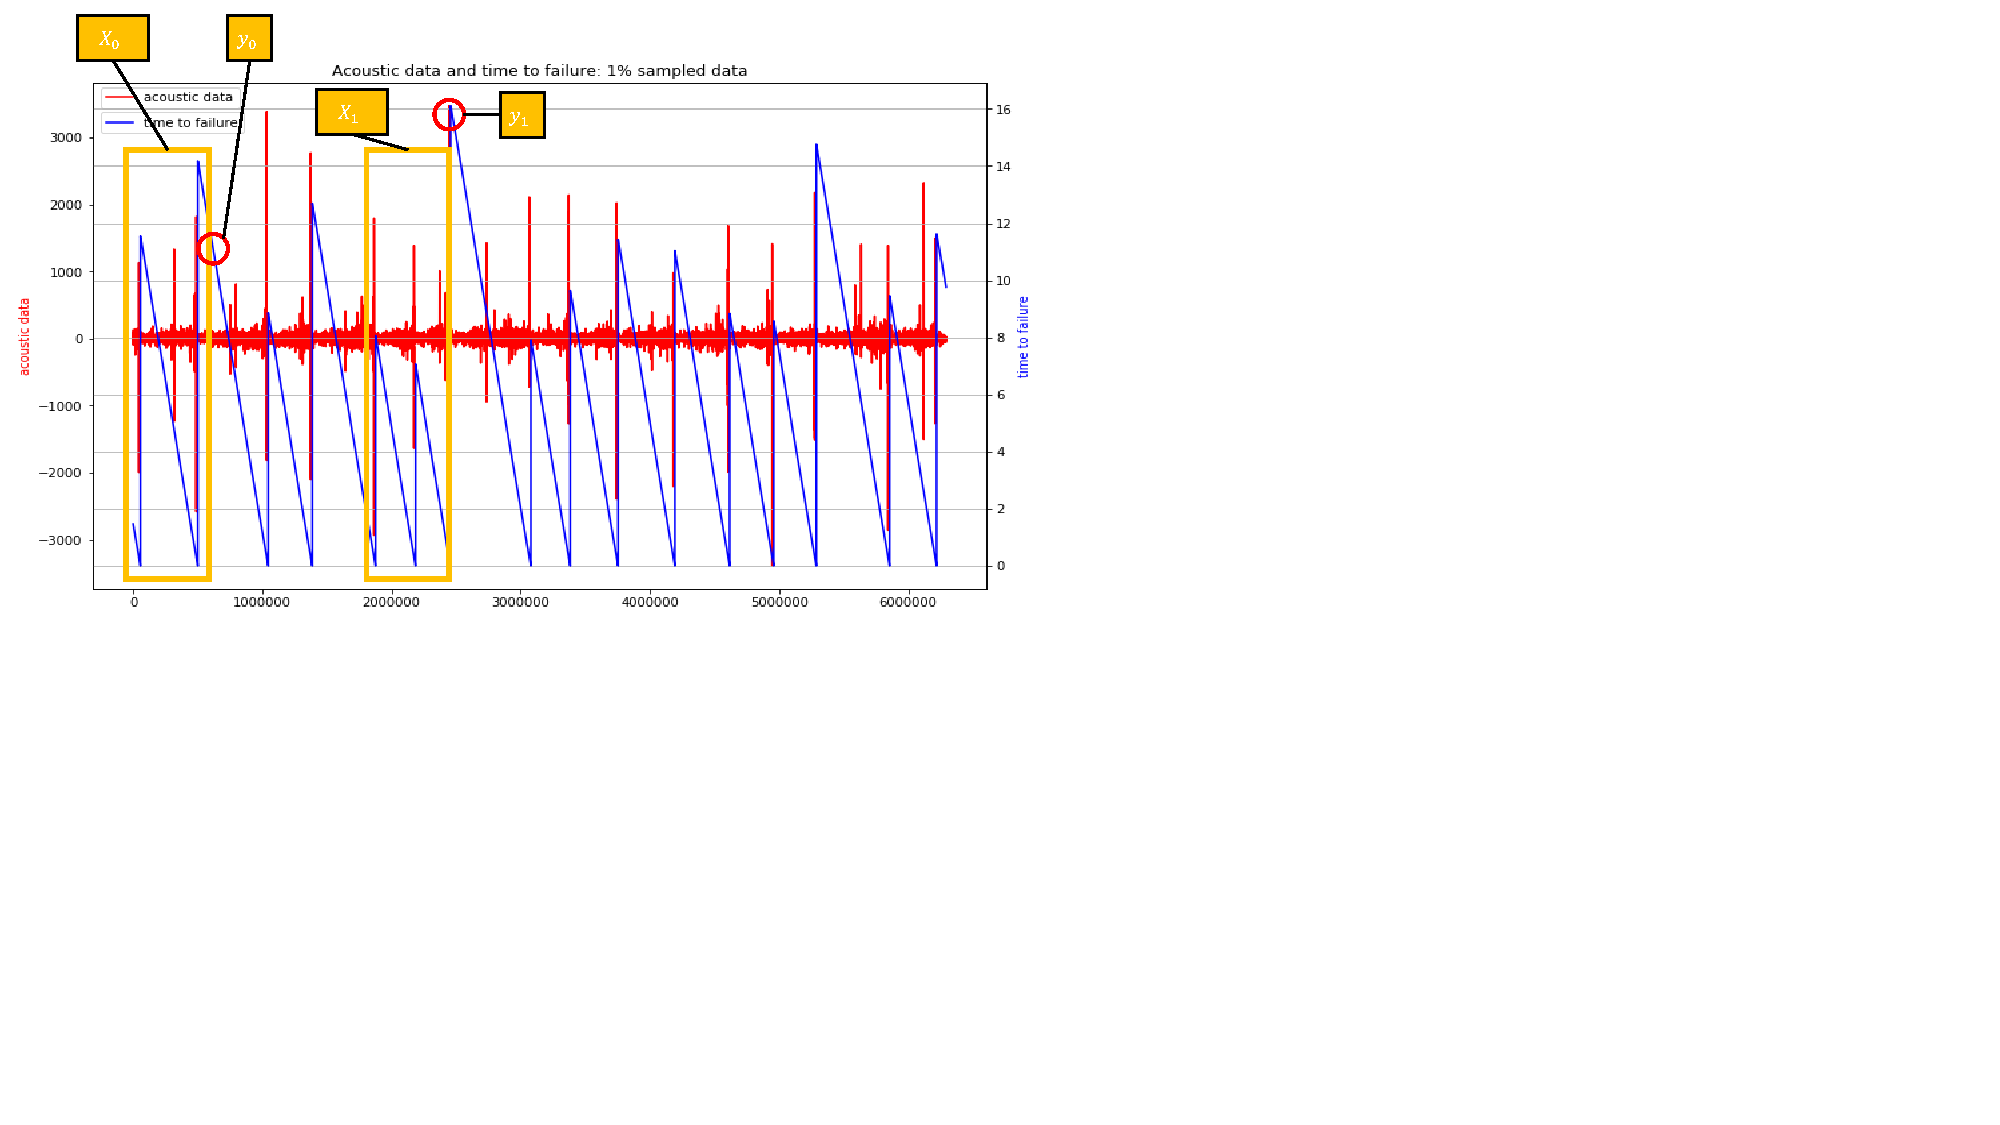
\includegraphics[width=2.9in]{graphs/data_slicing.pdf}
    \caption{Data feeding pipeline when training.}
    \label{fig:model_feeding_pipeline}
\end{figure}

\section{Sensor Data Augmentation}

As brought out before, we believe that with more data together, the model could learn better. Though these four data channels differ a little from each other, they approximately follow the same distribution. Hence, besides training the model on every single channel of \text{$PM_{2.5}$} data, we also \textbf{combined} all these channels' data together and fed it. The corresponding data is called \text{$PM_{2.5}$ (All)}.

\section{Experiments}
% 描述实验的组别,个数
As we sampled $PM_{2.5}$ data from 4 sensors, Sensor 0 to Sensor 3, so we have four channels of $PM_{2.5}$ IAQI data, and there are three different stride values. Finally, we have 12 experiments. Besides, we have a group of augmentation experiments in which all four sensors' data are fed to the model, yielding another three experiments.
% LR 配置
For each experiment, We optimized our GreenEyes model using Adam \cite{kingma2017adam} an initial learning rate of 0.0001, which is multiplied by 0.1 after 20 epochs. We trained our model to 100 epochs for each experiment.
% Loss 配置
We used mean squared error (MSE) as a loss metric and recorded mean absolute error (MAE). They are defined by equations below:

\begin{equation}
    MSE(p, y)=E((p_i-y_i)^2)
\end{equation}

\begin{equation}
    MAE(p, y)=E(|p_i-y_i|)
\end{equation}

Where $p$ is the prediction sequence and $y$ is the polygonized $PM_{2.5}$ IAQI sequence.

% four metrics, mean squared error (MSE), mean absolute percentage error (MAPE), mean squared logarithmic error (MSLE).

\subsection{Training and Validation} % 15 experiments

\subsubsection{Training Loss Curves}

Figure \ref{fig:training_mse} and Figure \ref{fig:val_mse} illustrate the training MSE curves and validation MSE curves respectively. It is observed that our system can fit the data well.
% \yan{Add a conclusion. } \yan{It is observed our system can xxx.}

% \yan{By the way, does your institution require inserting PDF figures?}

\begin{figure}[!htbp]
    \centering
    \begin{subfigure}[!htbp]{.45\textwidth}
        \centering
        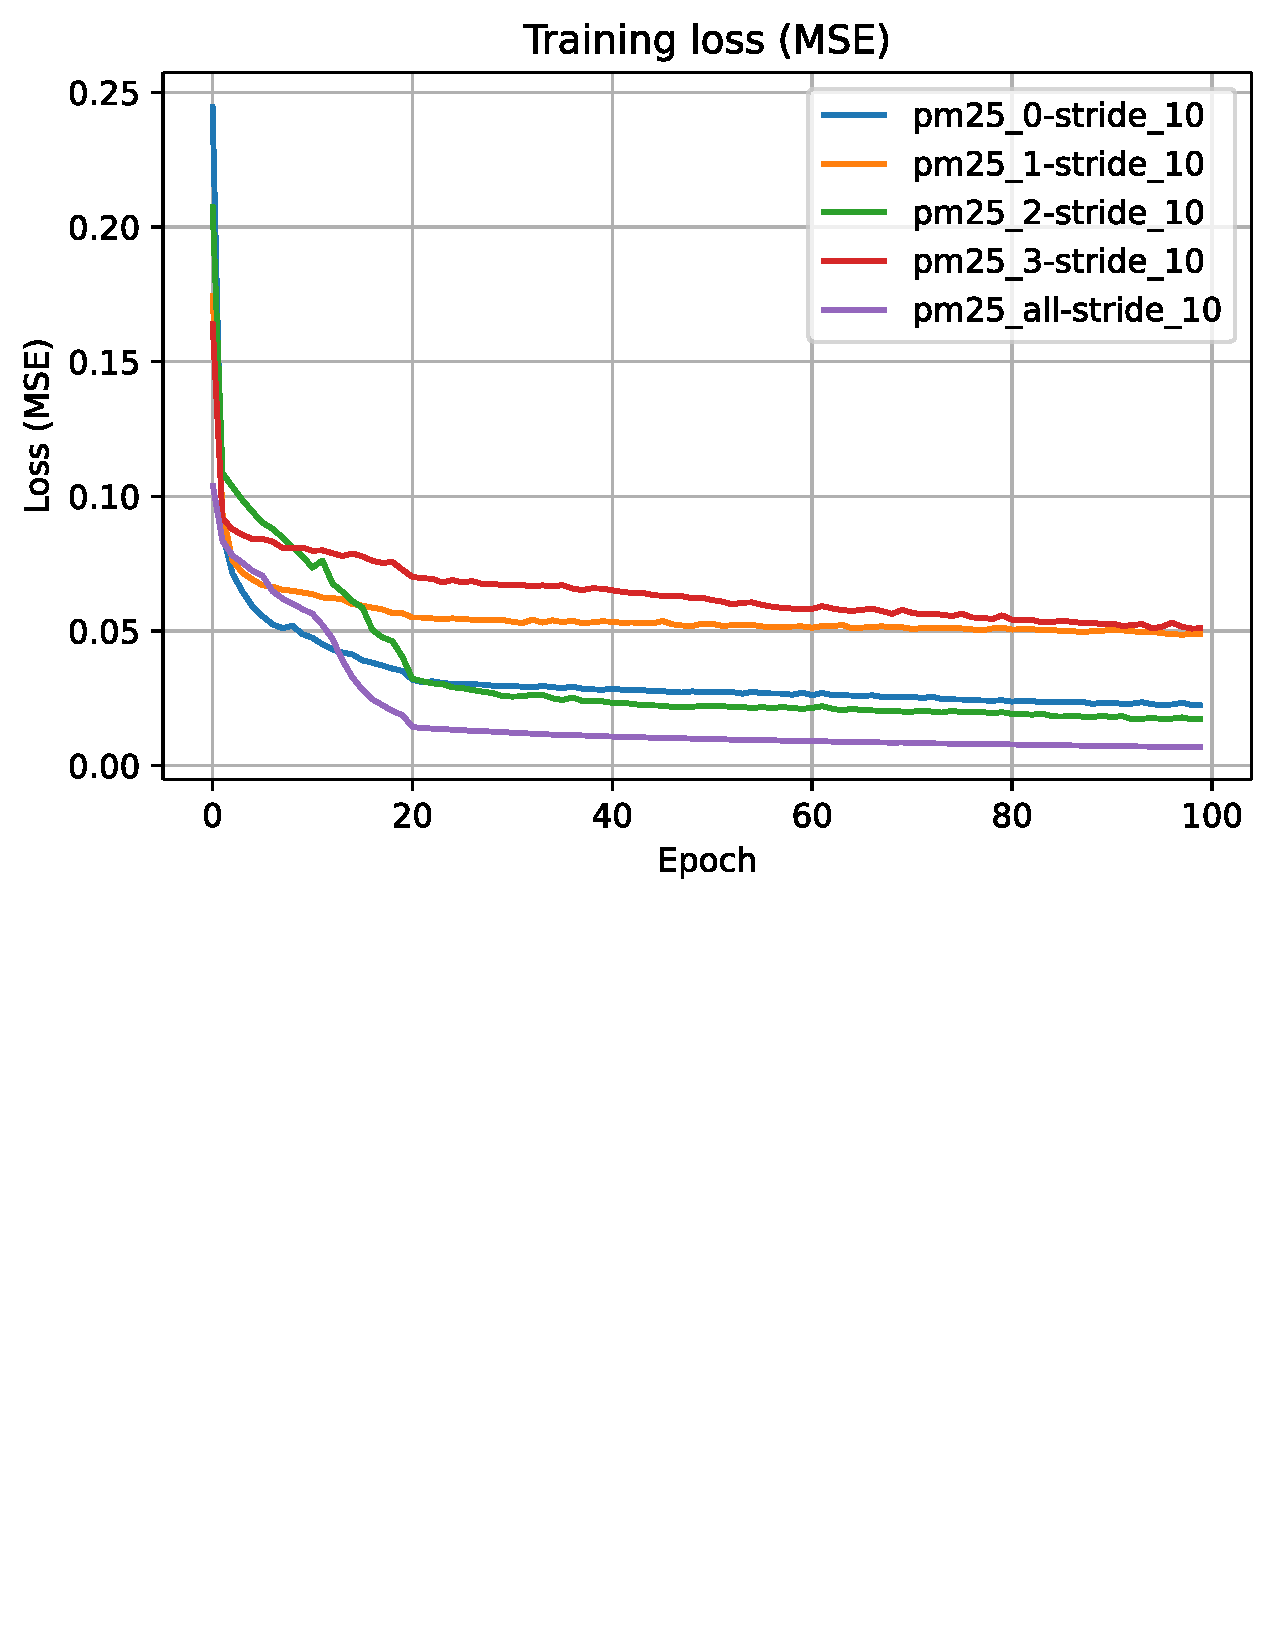
\includegraphics[width=\textwidth]{fig/results/train_curves_stride_10.pdf}
        \caption{stride=10.}
        \label{fig:train_stride_10}
    \end{subfigure}
    \hfill
    \begin{subfigure}[!htbp]{.45\textwidth}
        \centering
        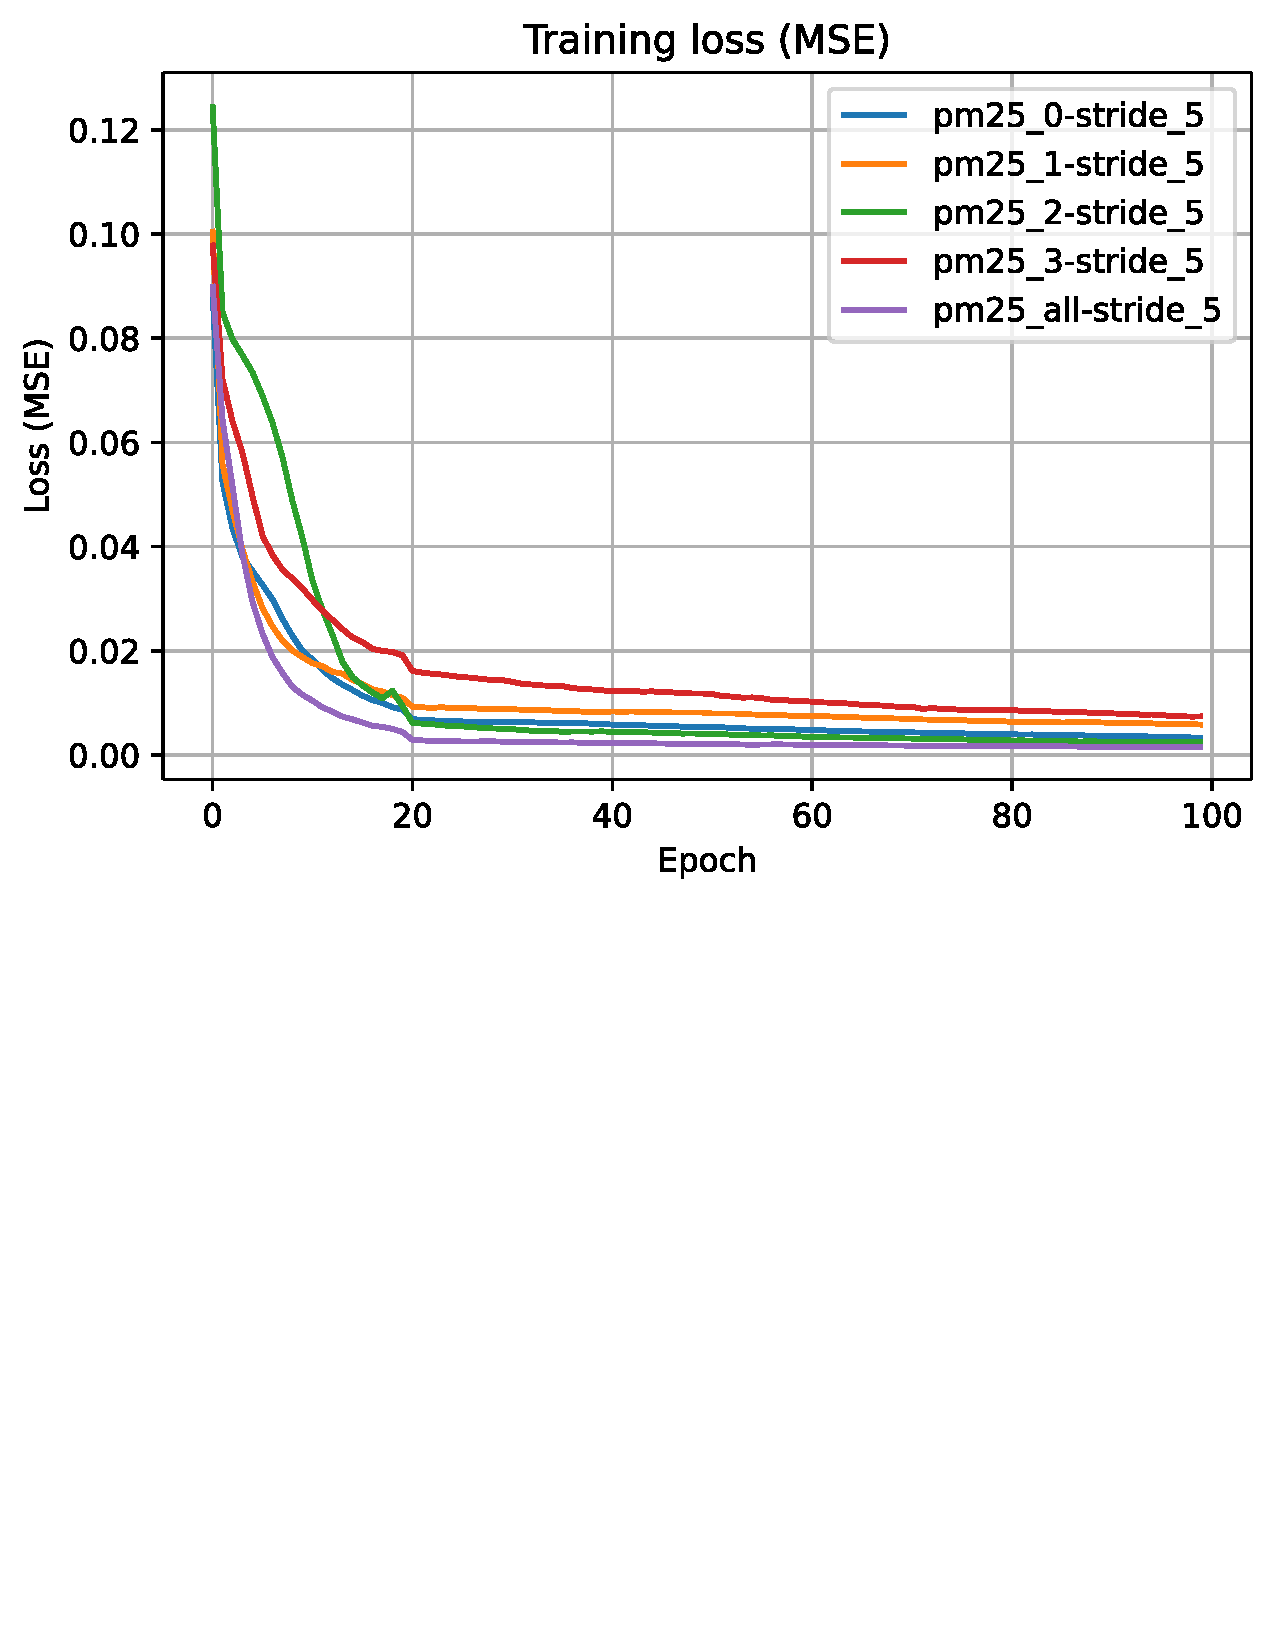
\includegraphics[width=\textwidth]{fig/results/train_curves_stride_5.pdf}
        \caption{stride=5.}
        \label{fig:train_stride_5}
    \end{subfigure}
    % \hfill
    \begin{subfigure}[!htbp]{.45\textwidth}
        \centering
        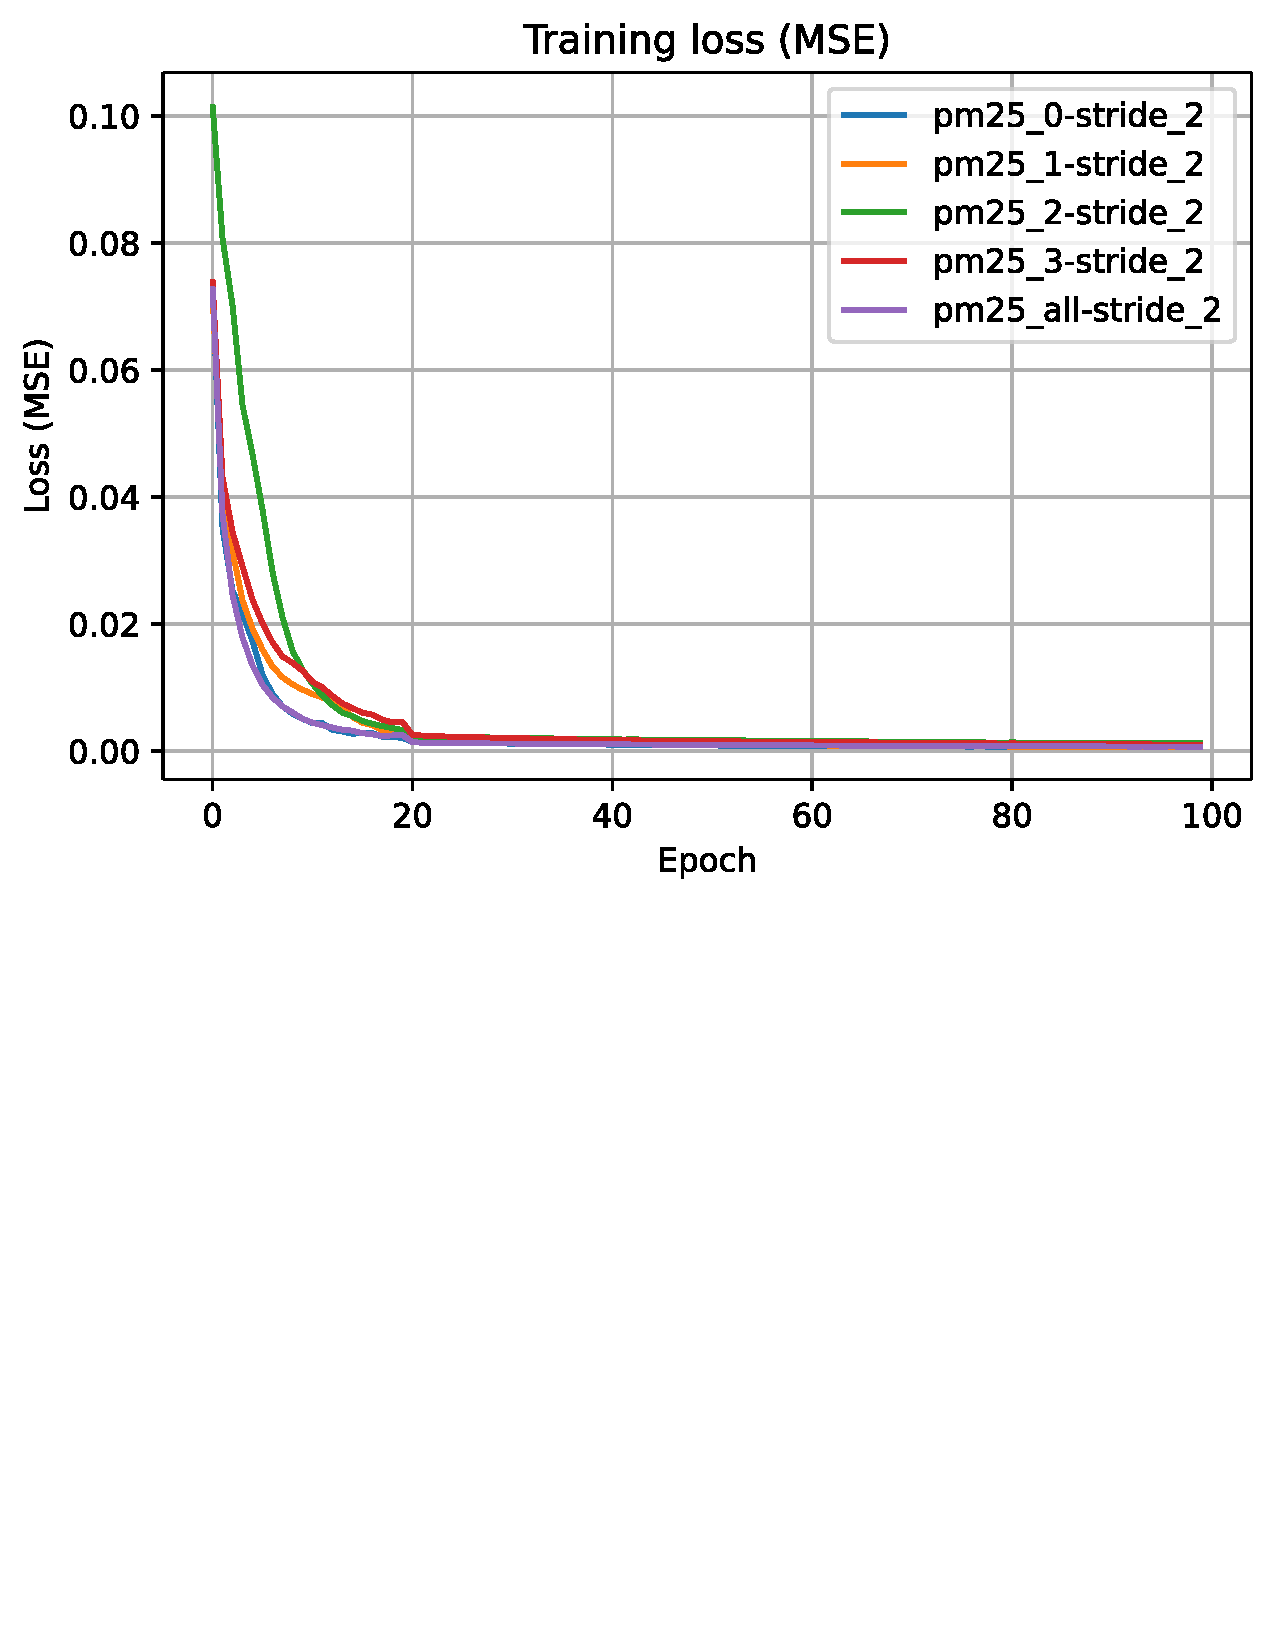
\includegraphics[width=\textwidth]{fig/results/train_curves_stride_2.pdf}
        \caption{stride=2.}
        \label{fig:train_stride_2}
    \end{subfigure}
\caption{Training MSE curves.}
\label{fig:training_mse}
\end{figure}

\begin{figure}[!htbp]
    \centering
    \begin{subfigure}[!htbp]{.45\textwidth}
        \centering
        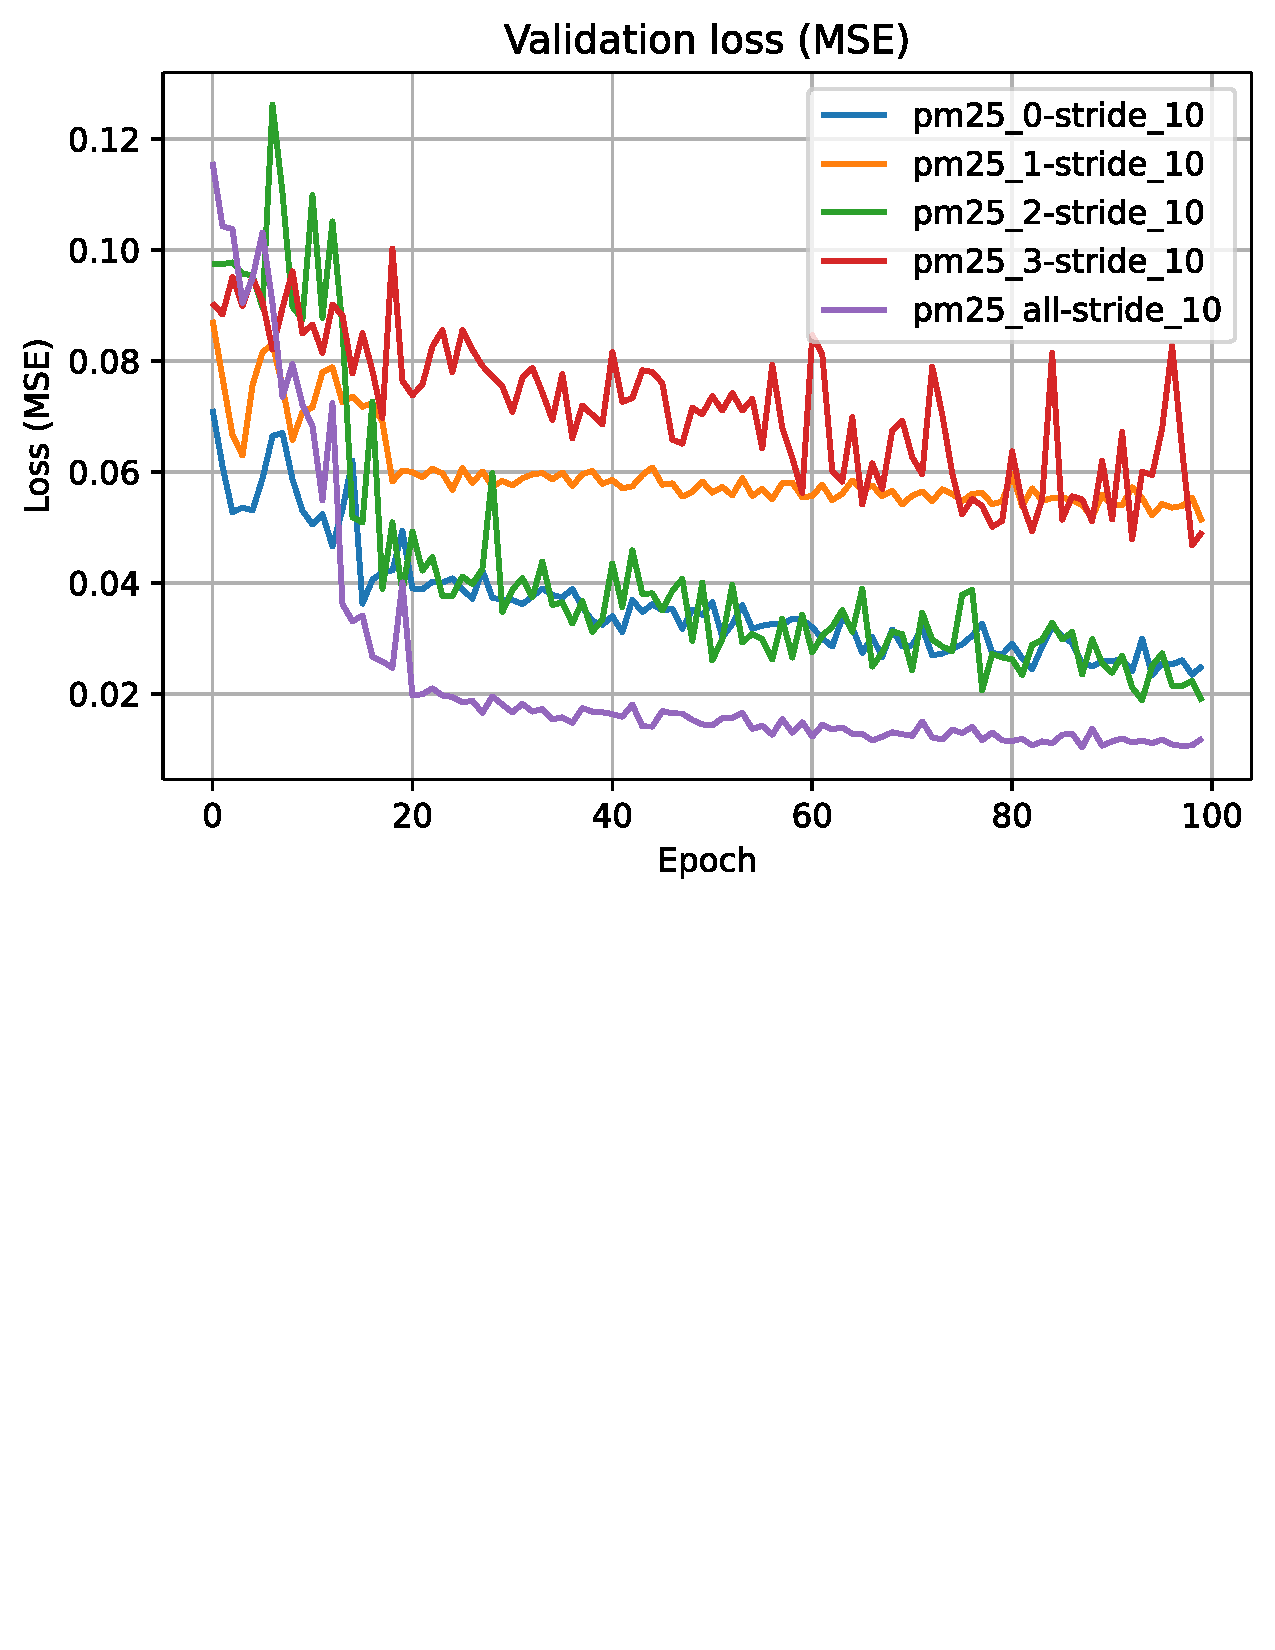
\includegraphics[width=\textwidth]{fig/results/val_curves_stride_10.pdf}
        \caption{stride=10.}
        \label{fig:val_stride_10}
    \end{subfigure}
    \hfill
    \begin{subfigure}[!htbp]{.45\textwidth}
        \centering
        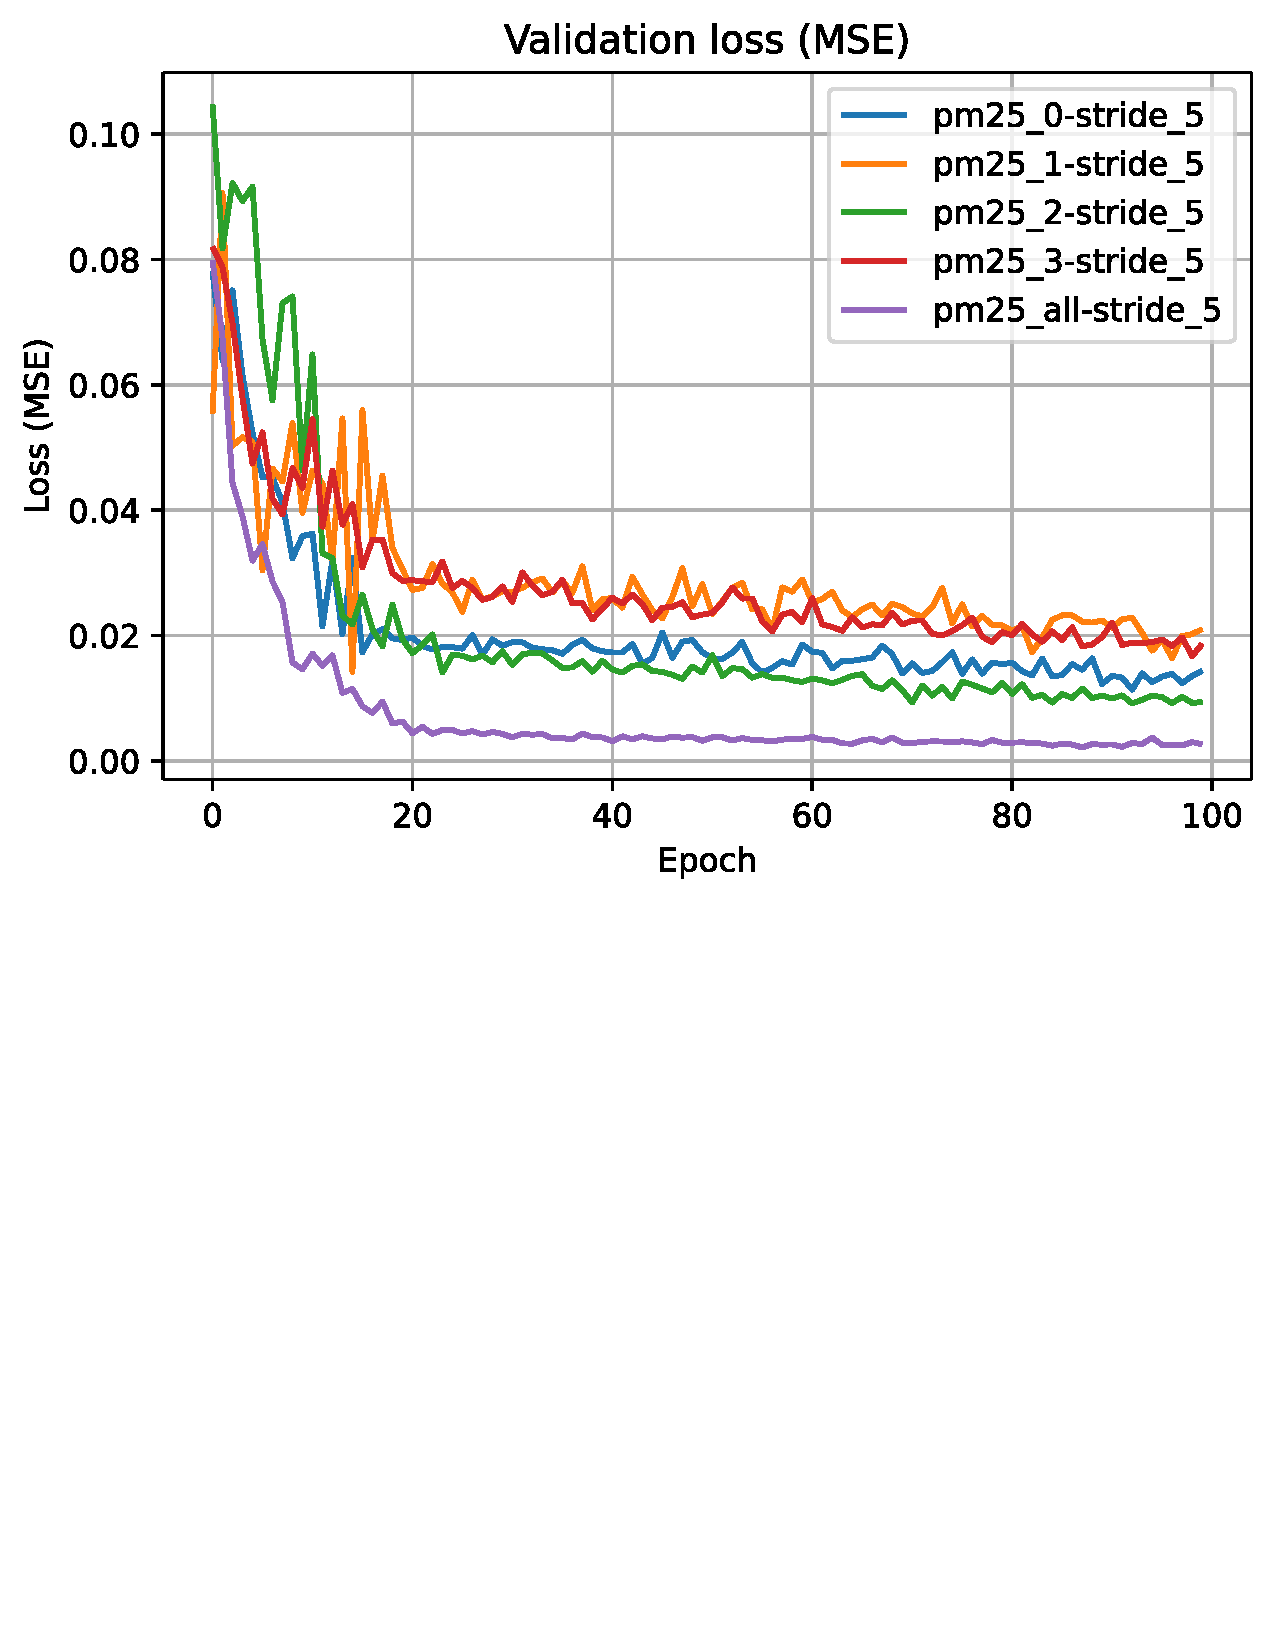
\includegraphics[width=\textwidth]{fig/results/val_curves_stride_5.pdf}
        \caption{stride=5.}
        \label{fig:val_stride_5}
    \end{subfigure}
    % \hfill
    \begin{subfigure}[!htbp]{.45\textwidth}
        \centering
        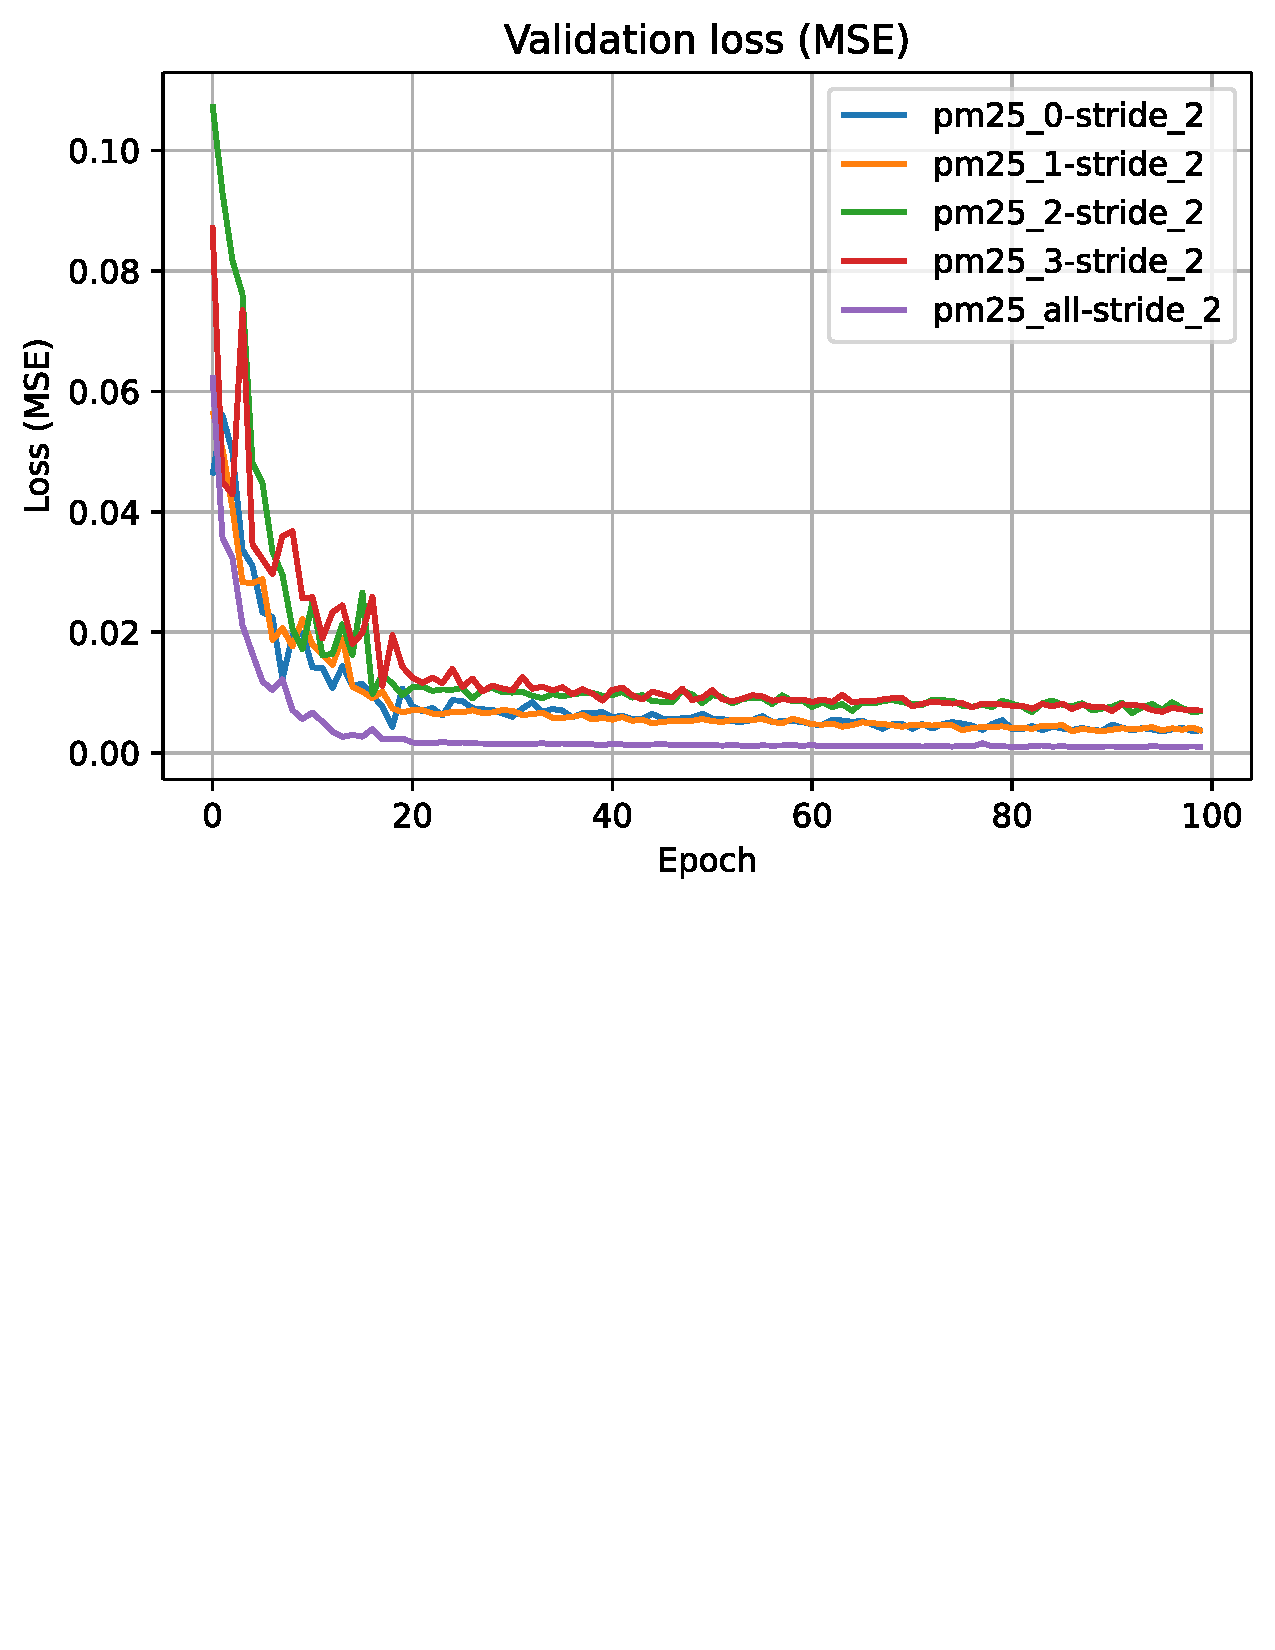
\includegraphics[width=\textwidth]{fig/results/val_curves_stride_2.pdf}
        \caption{stride=2.}
        \label{fig:val_stride_2}
    \end{subfigure}
\caption{Validation MSE curves.}
\label{fig:val_mse}
\end{figure}

% 讨论一个 Sensor,其它的放附录
% For Sensor 0, we fed the model with three different stride values. Figure
% the learning curves
% after the learning rate changes at the 20th epoch
% For more model training data, please refer to Appendix \ref{chapter:other_model_training_data}
% Figure \ref{fig:model_training_mse_mae_msle} shows the training process. We can infer that the model is already saturated after 100 epochs.

\subsubsection{Training Best Metrics}

As we used MSE as loss, i.e., the supervising metric, we extracted minimum train MSE and minimum validation MSE from all the training epochs. These best metric results reflect the model's fitting capability. They are all rounded to 4 decimals. 

% We also record other metrics such as MAE during training.

Table \ref{table:best_metrics} lists each experiment's final best metrics during training.

\begin{table}[!htbp]
    \centering
    \begin{tabular}{|c|c|c|c|c|}
        \hline\hline
        Data & Stride & Minimum train MSE & Minimum validation MSE & ratio \\\hline
        \multirow{3}{*}{\text{$PM_{2.5}$(0)}} & 10 & 0.0223 & 0.0234 & 0.96 \\ \cline{2-5} 
                                        & 5 & 0.0034 & 0.0114 & 0.30 \\ \cline{2-5} 
                                        & 2 & \textbf{\textit{0.0006}} & \textbf{\textit{0.0035}} & 0.16 \\ \hline
        \multirow{3}{*}{\text{$PM_{2.5}$(1)}} & 10 & 0.0486 & 0.0510 & 0.95 \\ \cline{2-5} 
                                        & 5 & 0.0058 & 0.0142 & 0.41 \\ \cline{2-5} 
                                        & 2 & \textbf{\textit{0.0006}} & \textbf{\textit{0.0036}} & 0.17 \\ \hline
        \multirow{3}{*}{\text{$PM_{2.5}$(2)}} & 10 & 0.0171 & 0.0187 & 0.92 \\ \cline{2-5} 
                                        & 5 & 0.0024 & 0.0092 & 0.27 \\ \cline{2-5} 
                                        & 2 & \textbf{\textit{0.0012}} & \textbf{\textit{0.0066}} & 0.19 \\ \hline
        \multirow{3}{*}{\text{$PM_{2.5}$(3)}} & 10 & 0.0509 & 0.0468 & 1.09 \\ \cline{2-5} 
                                        & 5 & 0.0074 & 0.0167 & 0.44 \\ \cline{2-5} 
                                        & 2 & \textbf{\textit{0.0010}} & \textbf{\textit{0.0068}} & 0.15 \\ \hline
        \multirow{3}{*}{\text{$PM_{2.5}$(All)}} & 10 & 0.0068 & 0.0103 & 0.66 \\ \cline{2-5} 
                                        & 5 & 0.0014 & 0.0022 & 0.67 \\ \cline{2-5} 
                                        & 2 & \textbf{0.0007} & \textbf{0.0009} & 0.77 \\
        \hline
        \hline
    \end{tabular}
    \caption{Experiments' final best metrics.}
    \label{table:best_metrics}
\end{table}

We also define a generalization coefficient ratio as the equation below to measure the model's generalization capability during certain experiments. The larger the ratio,  the better the generalization capability is. The ratio results are rounded to 2 decimals.

\begin{equation}
    ratio=\frac{min(train\ MSE)}{min(validation\ MSE)}
\end{equation}

\subsection{Model Evaluation}

% Evaluation curves
\begin{figure}
    \centering
    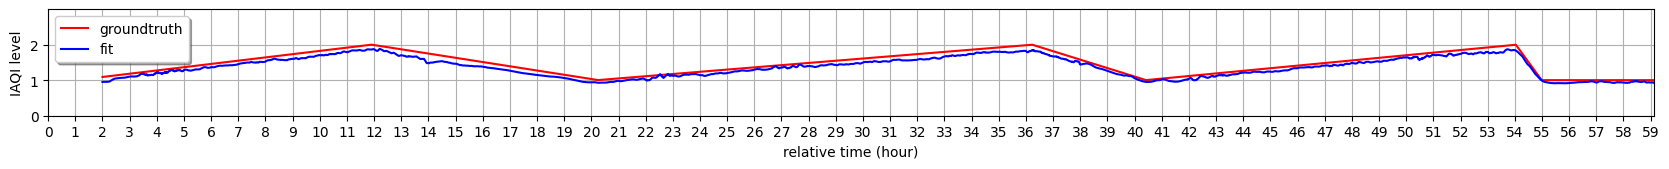
\includegraphics[width=\linewidth]{fig/model_eval_pm25_0_stride_10.png}
    \caption{Evaluation of the GreenEyes model (\text{$PM_{2.5} (0)$}, stride=10).}
    \label{fig:model_eval_pm25_0_stride_10}
\end{figure}

As earthquake prediction aims to fit the model and learn time-series information, i.e., the triangular lines in coordination with the acoustic data, our model also fits the level lines regarding their air pollutant concentration data. Figure \ref{fig:model_eval_pm25_0_stride_10} proves that the model fits the labeled IAQI level lines well, except that its predictions differ from the ground truth a little on some parts of the lines, and especially on the turning corners of the piecewise linear function.

% Test results table here.
To quantify the testing results of our model by different parameters, we tested it on the whole $PM_{2.5}$ sequence by setting stride as 1, which is different from the training config. As stride is set to 1, the slice window will move one point after another. Hence, the model can make the inference on the whole source sensor data. When the stride is set a 10, 5, and 2 for different training data sampling configs, these sampled data slices form a subset of the sliced data when the stride is set to 1.

We performed the tests using two metrics, mean square error (MSE) and mean absolute error (MAE).

And we test all models trained under different stride parameters and on every channel of $PM_{2.5}$ data. Table \ref{table:test_mse_mae} lists the statistics of our tests. Digit in the brackets is the channel number. "All" means the model is trained by all channels together. All result values of MSE have rounded four decimals, and all MAE values are rounded to 2 decimals.

\begin{table}[!htbp]
    \centering
    \begin{tabular}{|c|c|c|c|}
        \hline\hline
        Data & Stride & MSE & MAE \\\hline
        \multirow{3}{*}{\text{$PM_{2.5}$(0)}} & 10 & 0.0266 & 0.13 \\ \cline{2-4} 
                                        & 5 & 0.0144 & 0.11 \\ \cline{2-4} 
                                        & 2 & \textbf{\textit{0.0037}} & \textbf{\textit{0.05}} \\ \hline
        \multirow{3}{*}{\text{$PM_{2.5}$(1)}} & 10 & 0.0517 & 0.18 \\ \cline{2-4} 
                                        & 5 & 0.0113 & 0.10 \\ \cline{2-4} 
                                        & 2 & \textbf{\textit{0.0036}} & \textbf{\textit{0.05}} \\ \hline
        \multirow{3}{*}{\text{$PM_{2.5}$(2)}} & 10 & 0.0188 & 0.11 \\ \cline{2-4} 
                                        & 5 & 0.0092 & 0.09 \\ \cline{2-4} 
                                        & 2 & \textbf{\textit{0.0069}} & \textbf{\textit{0.07}} \\ \hline
        \multirow{3}{*}{\text{$PM_{2.5}$(3)}} & 10 & 0.0501 & 0.16 \\ \cline{2-4} 
                                        & 5 & 0.0108 & 0.09 \\ \cline{2-4} 
                                        & 2 & \textbf{\textit{0.0070}} & \textbf{\textit{0.07}} \\ \hline
        \multirow{3}{*}{\text{$PM_{2.5}$(All)}} & 10 & 0.0118 & 0.09 \\ \cline{2-4} 
                                        & 5 & 0.0026 & 0.04 \\ \cline{2-4} 
                                        & 2 & \textbf{0.0010} & \textbf{0.02} \\ \hline
        \hline
        \hline

    \end{tabular}
    \caption{Test MSE and MAE under different strides.}
    \label{table:test_mse_mae}
\end{table}

The data on the table shows that for each channel of $PM_{2.5}$ data, the smaller the stride parameter is, the less the MSE and MAE are, which means the model can fit the target better. This is reasonable and consistent with our intuition.

Meanwhile, when put all channels' data together and feed the model, it can learn the best result.

Figure \ref{fig:test_mse} and Figure \ref{fig:test_mae} respectively present the test MSE and MAE results by bar plots. The plots are divided into three stride groups, which's stride is 10, 5, 2. Results from the different data channels (or all channels of the data) but sharing the same stride join into the same group for comparisons.

\begin{figure}[!htbp]
    \centering
    \begin{subfigure}[!htbp]{.45\textwidth}
        \centering
        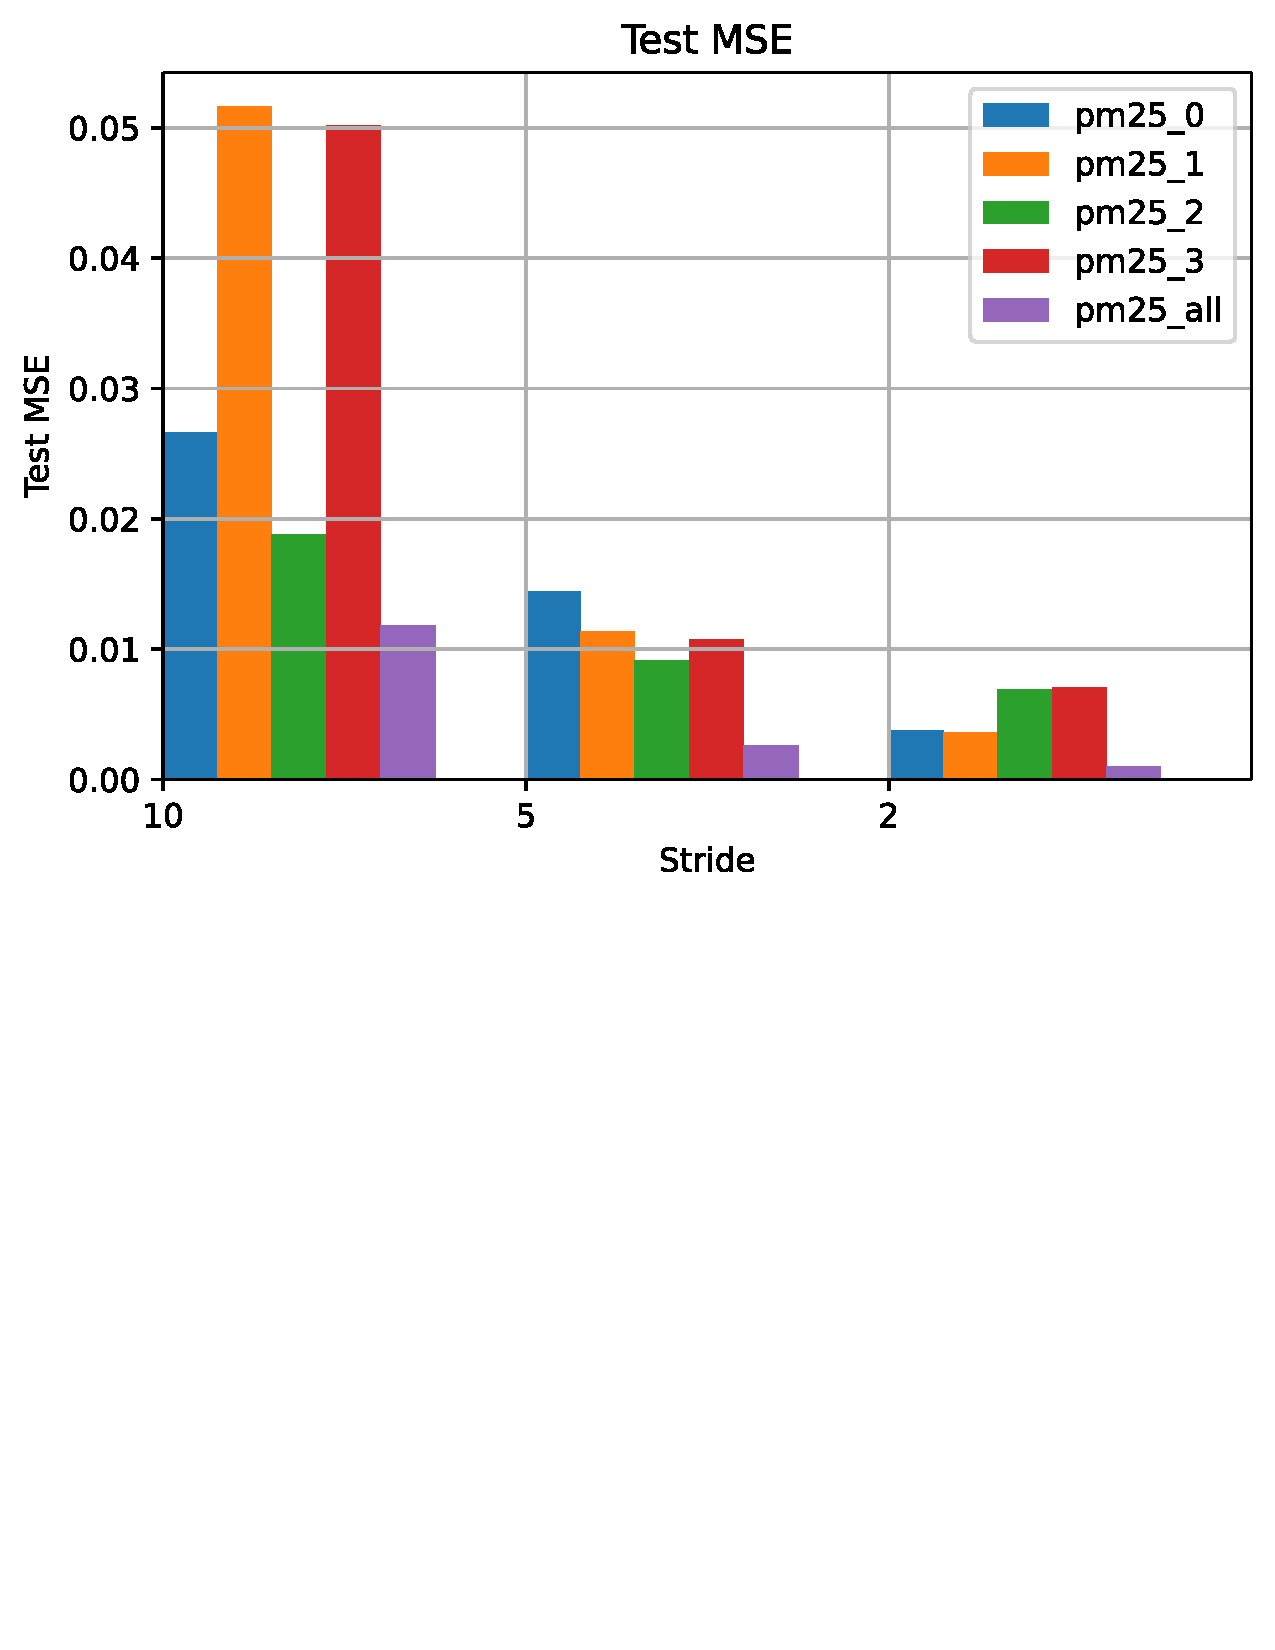
\includegraphics[width=\textwidth]{fig/results/test_mse.pdf}
        \caption{Test MSE.}
        \label{fig:test_mse}
    \end{subfigure}
    \begin{subfigure}[!htbp]{.45\textwidth}
        \centering
        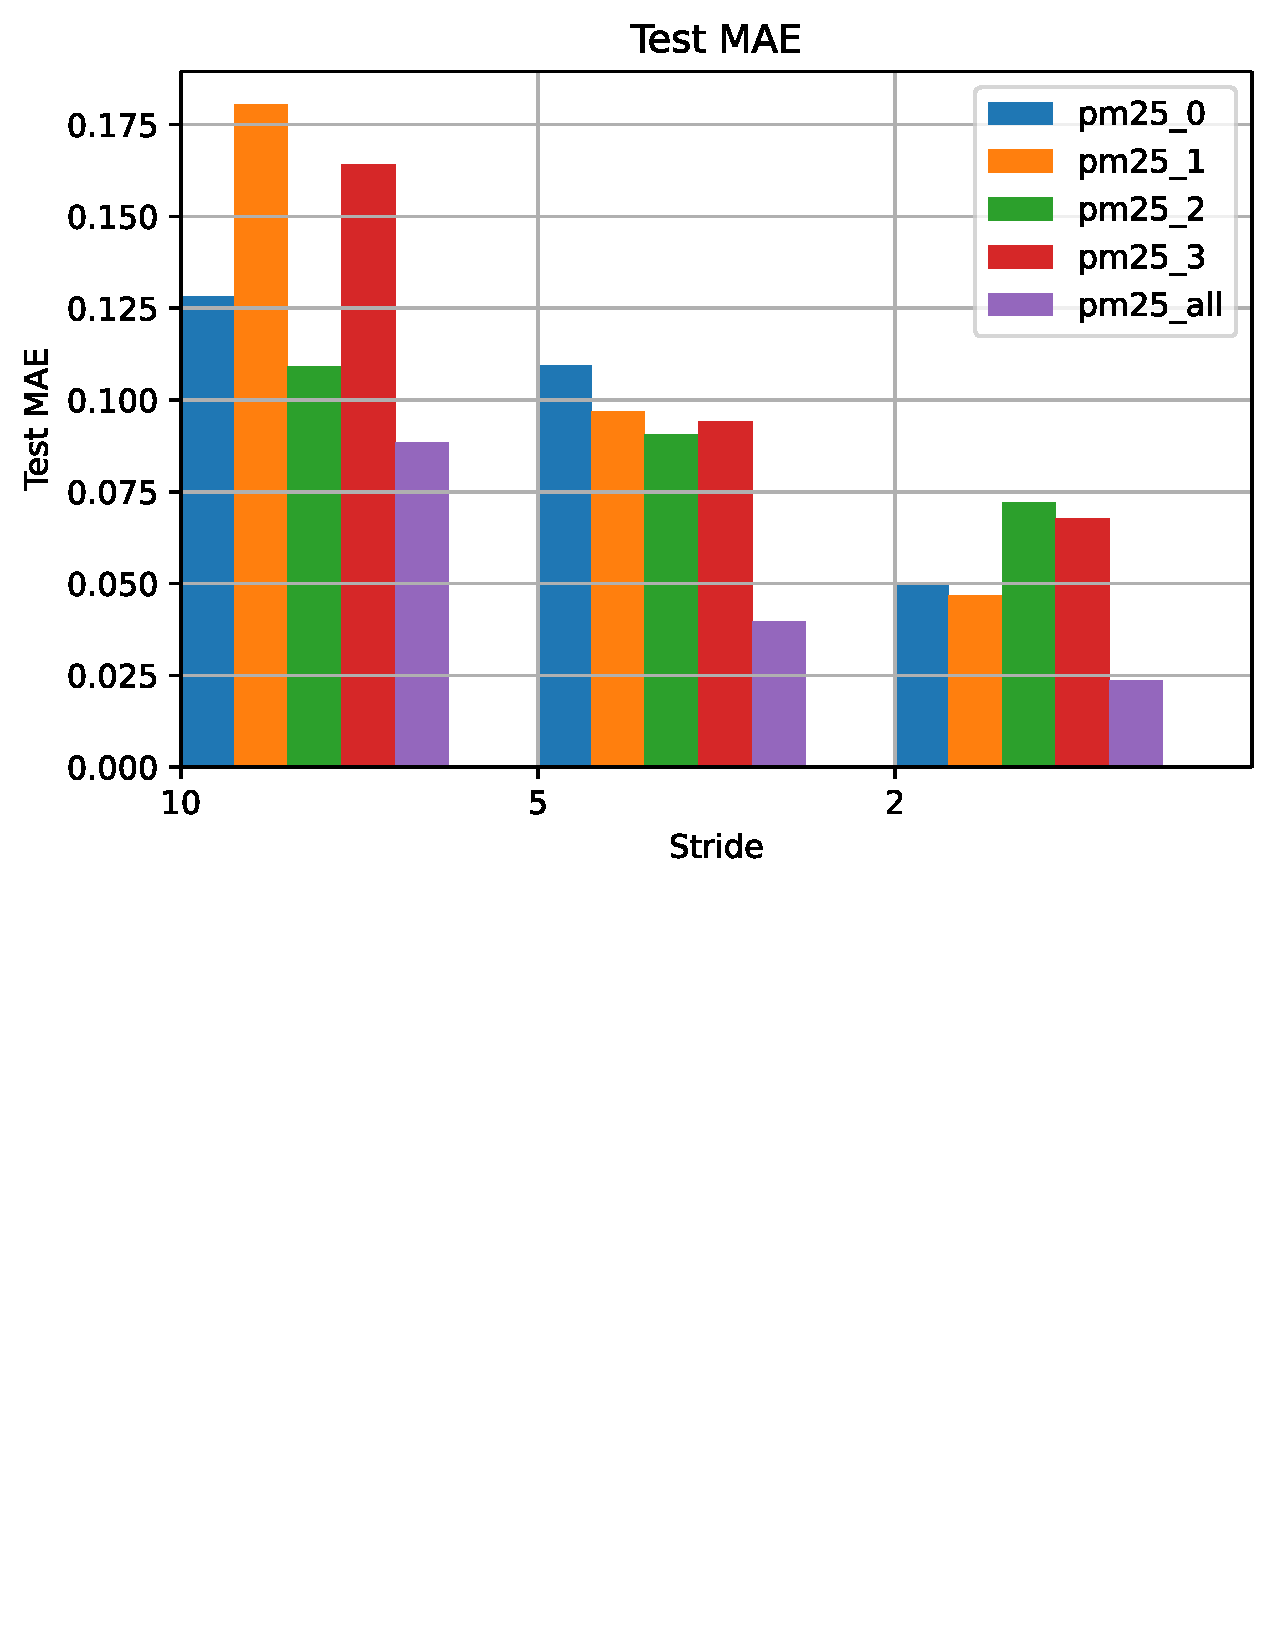
\includegraphics[width=\textwidth]{fig/results/test_mae.pdf}
        \caption{Test MAE.}
        \label{fig:test_mae}
    \end{subfigure}
    \caption{Test MSE and MAE.}
    \label{fig:test_mse_mae}
\end{figure}

\subsection{Results Analyses}

From the results table and bar plots, we could draw at least two useful and meaningful conclusions. Firstly, for each kind of data, whichever $PM_{2.5}$ (i) or $PM_{2.5}$ (All), when the stride parameter decreases, the model can outcome better results.

Secondly, in each stride group, $PM_{2.5}$ (All)'s performance surpasses every single channel of $PM_{2.5}$ data, w.r.t. both MSE and MAE. And when the stride is 5 or 2, this conclusion is more significant.

The first conclusion is obvious. As Table \ref{table:N_samples} shows, the smaller the stride is, the number of training samples gets larger. More data will result in a better model's fitting performance. However, while we want the model to predict and fit more precisely, we don't want to sample sliced data from original data flow too frequently (set the stride too small). The model's capability is reflected by its relevant fitting results (MSE, MAE, etc.), while a rather less frequent sampling is configured (e.g., set stride to 10, not 2).

For our GreenEyes model, the evaluation curve in Figure \ref{fig:model_eval_pm25_0_stride_10} shows its fitting capability, as stride 10 is already enough.

During application, we could trade off on this stride parameter to balance the model's performance and the computation costs.
